% !TeX root = ../main.tex

\chapter{系统概要设计}

\section{系统概述}
本章在需求分析的基础上,对RISC-V指令集模拟器的整体架构设计进行阐述,并对各功能模块进行分析建模,在本章节的基础上,可以从整体上了解RISC-V指令集模拟器的设计思路,为后续的具体实现提供指导。


\section{系统静态结构}
本系统是针对RISC-V芯片开发团队在系统软件开发和移植过程中使用的体系结构模拟器。用户将编译好的RISC-V架构可执行程序加载到模拟器上运行,控制执行流程,观察执行结果,能够脱离实际硬件平台进行系统软件的调试。该RISC-V指令集模拟器的整体功能模块如图\ref{fig:sim_general}所示,主要包含四个功能模块:预加载模块,CPU和总线模块,中断控制器模块,以及调试和UI模块。其中,预加载模块包括模拟器参数配置,指令集注册,加载ELF文件功能;CPU和总线模块包括了核心的处理器模拟,内存模拟,总线模拟等功能,是模拟器的主体功能模块;中断控制器模块包括PLIC模拟和部分外设模拟;调试模块包含了断点设置,内存查询,模拟中断信号发送功能,和UI显示模块结合在一起,提供目标程序执行窗口,调试窗口等的可视化界面和模拟器状态查询功能。
\begin{figure}[H]
  \centering
  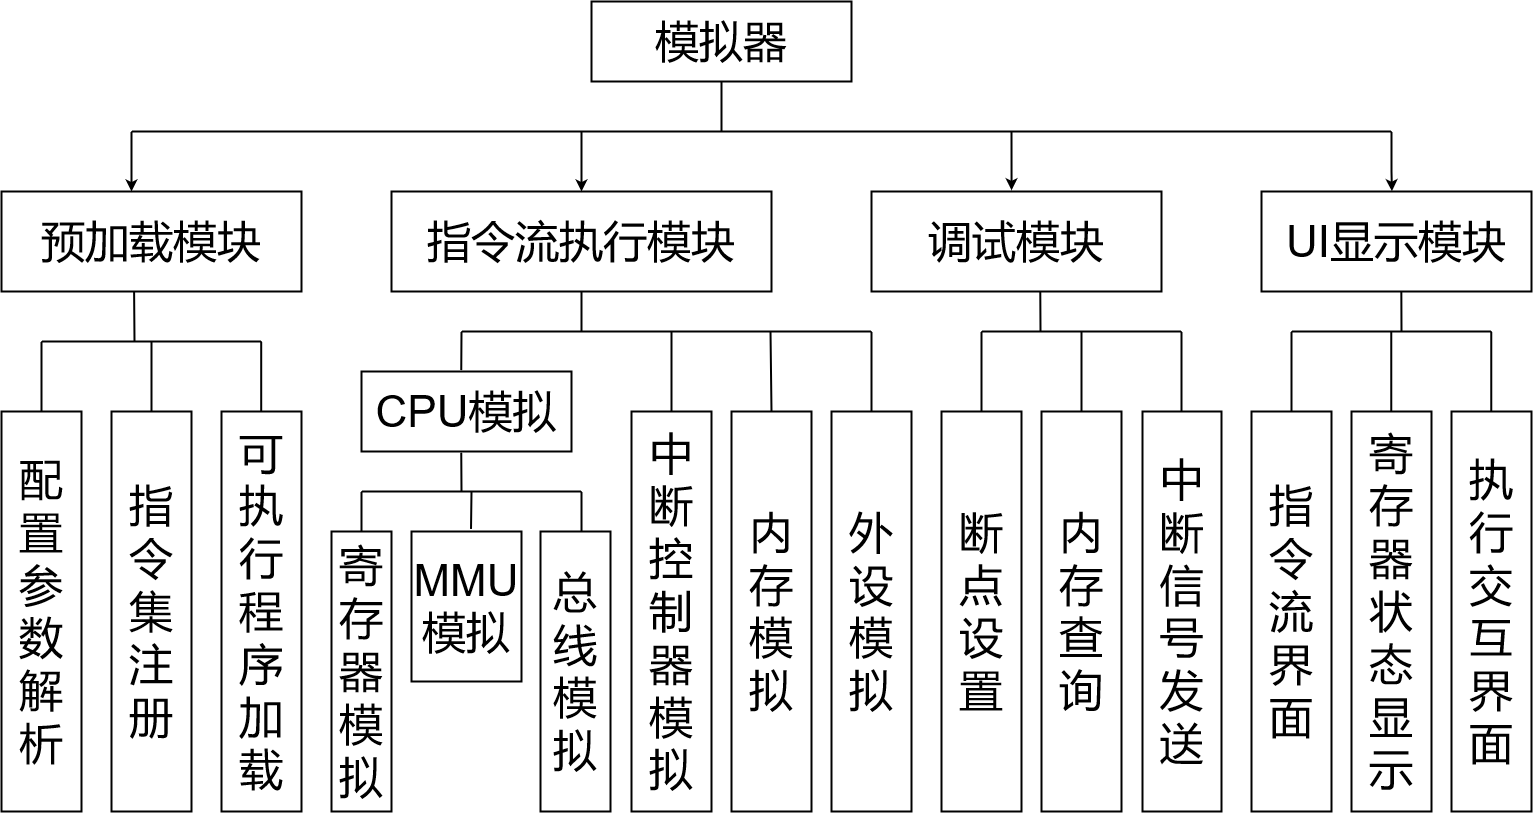
\includegraphics[width=0.9\textwidth]{sim-general.png}
  \caption{系统功能模块图}
  \label{fig:sim_general}
\end{figure}


根据模拟器各个功能模块的特点和业务需求,确定了RISC-V指令集模拟器的整体层次架构如图\ref{fig:structure}所示,共分为5层。硬件层主要是X86架构的宿主机环境。数据层主要包括RISC-V目标程序二进制文件,和注册过相应指令集模块的译码器。在模拟器运行时还包括动态的缓存及主存模拟数据。逻辑层包含了模拟器的业务处理逻辑,由预加载模块从数据层提取可执行代码,通过译码器进行翻译,CPU和总线模块执行相应的功能函数,最后将目标程序执行结果以及硬件状态变更同步到表现层。表现层主要由调试窗口,查询窗口和目标程序交互窗口组成。用于展示RISC-V目标程序执行结果,查询模拟器状态信息,以及提供交互调试界面。最终在用户层向用户提供完整的RISC-V指令集功能模拟器。


\begin{figure}[H]
  \centering
  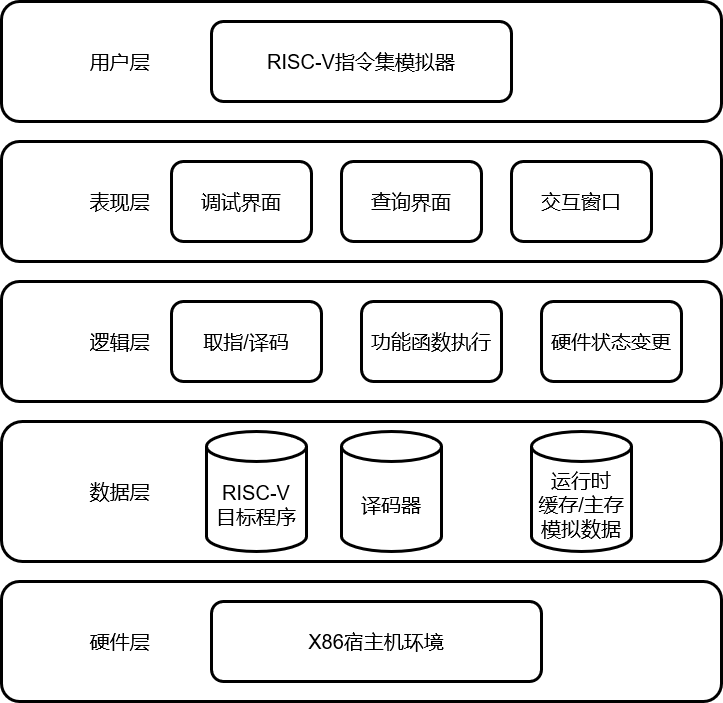
\includegraphics[width=0.8\textwidth]{cengci.png}
  \caption{系统整体架构图}
  \label{fig:structure}
\end{figure}


CPU和总线模块是模拟器的主体功能模块,该模块模拟了单条指令执行过程中的主要硬件行为,包括寄存器,MMU,高速缓存,主存,总线等。每个处理器都有独立的寄存器组,内存管理单元,所有处理器共享同一个iCache,dCache,紧随其后的是L2Cache和主存。模拟出的RISC-V CPU整体逻辑架构图如图\ref{fig:cpu}所示,从图中可以看出,模拟器以单个处理器(在RISC-V架构中称为硬件线程Hart)为核心模拟对象,核内的数据通信不经过总线,直接在处理器复合类对象内部进行通信,具体的类图见下一章。所有内存映射I/O(Memory-Mapped I/O, MMIO)都需要经过总线,包括时钟,Bootrom,平台级中断控制器以及调试模块。
\begin{figure}[H]
  \centering
  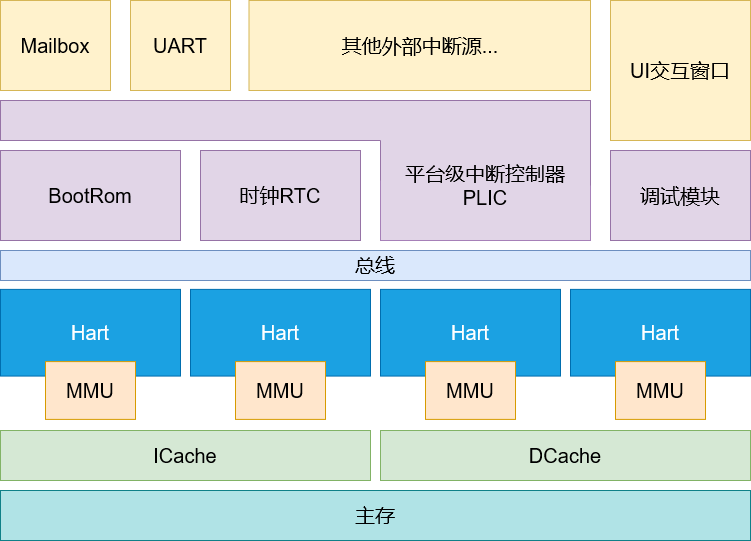
\includegraphics[width=0.8\textwidth]{cpu.png}
  \caption{处理器逻辑架构图}
  \label{fig:cpu}
\end{figure}


中断系统以平台级中断控制器(Platform-Level Interrupt Controller, PLIC)为核心,PLIC对外部中断源进行优先级裁决,对内表现为黑盒,处理器不需要关心具体的外部中断源情况,在接受外部中断信号时才会读取相应的外部中断ID,执行对应的中断处理程序。PLIC与处理器核的关系如图~\ref{fig:plic-to-hart}所示。在实际的硬件设计中,PLIC与每个处理器核都有两条硬连线,分别对应机器模式外部中断信号和监管模式外部中断信号。
\begin{figure}[H]
  \centering
  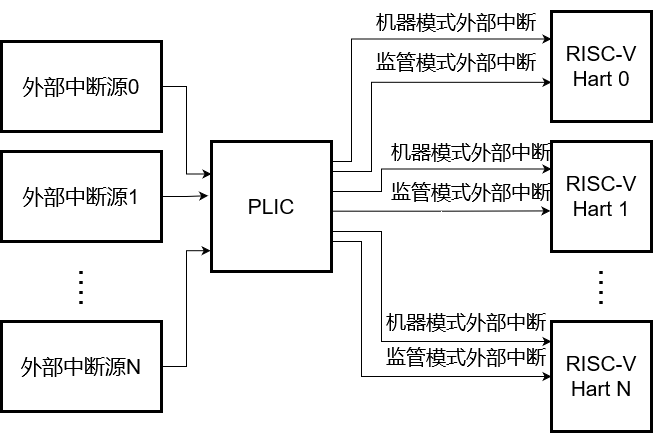
\includegraphics[width=0.8\textwidth]{plic_hart.png}
  \caption{PLIC外部中断}
  \label{fig:plic-to-hart}
\end{figure}


调试和UI模块的设计主要包含前端窗口设计,以及前后端对象间通信设计。前端窗口对象包含交互窗口,调试窗口和状态查询窗口,其中交互窗口需要模拟UART串口控制器,将交互窗口的键入复制到UART的FIFO队列,然后发起UART外部中断,通过PLIC和总线与处理器进行通信。该部分的设计使用了QWidget提供的"信号槽"机制,处理对象间的通信。只需要绑定自定义的信号函数和槽函数,就能方便地实现对象间的异步通信。详细的实现将在下一章进行阐述。

% \clearpage
\section{系统动态结构}
本模拟器是提供指令级别仿真的功能模拟器,模拟器单条指令运行的活动图如图~\ref{fig:sim-seq1}所示。
\begin{figure}[H]
  \centering
  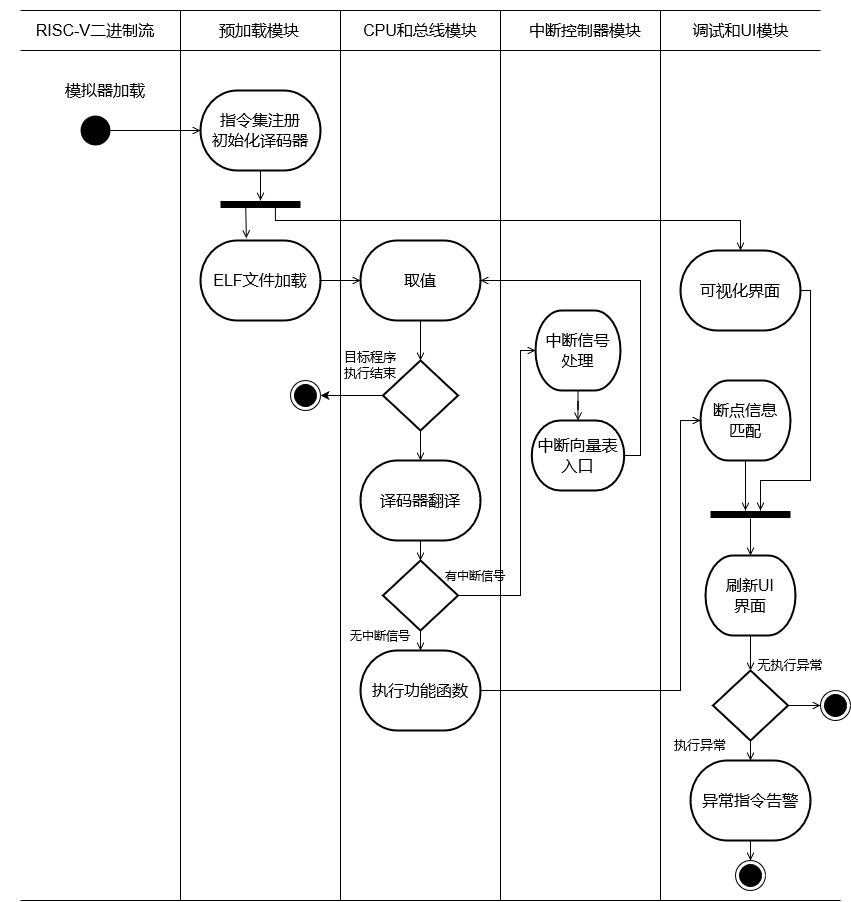
\includegraphics[width=1.0\textwidth]{huodong.png}
  \caption{模拟器执行单条指令活动图}
  \label{fig:sim-seq1}
\end{figure}


首先使用RISC-V交叉编译工具链将目标程序编译为RISC-V架构的ELF文件,然后模拟器解析该二进制文件,将对应的指令流搬运到BootROM,模拟器在配置启动后为处理器注册指令集,绑定解码器,逐条进行译码,执行。指令译码器完成包括操作数在内的指令信息提取,找到该条指令注册时对应的功能函数,执行该功能函数,然后将更新后的寄存器状态信息,内存状态信息同步到前端UI显示模块。在模拟器运行的过程中,用户还可以通过前端交互调试窗口来切换模拟器运行模式,设置断点触发条件,进行单步调试,状态查询等操作。


\subsection{解码器与指令集功能函数}
本模拟器实现了RISC-V特权指令集V1.9版本,和用户指令集V2.1版本的标准拓展指令集共196条指令的模拟。该部分模拟的核心是RISC-V汇编指令对应的功能函数,所有功能函数的实现都需要参照硬件设计团队的HDL代码,本项目使用了Chisel高级硬件设计语言进行芯片设计,无须对冗长复杂的Verilog代码进行抽象,能够方便地进行指令功能函数的编写。


模拟器启动后首先根据配置参数解析需要加载的指令集模块,然后遍历各个模块的指令列表,将指令操作码格式和对应的功能函数注册到译码器当中,作为模拟目标机器的完备指令集,后续的目标函数执行过程均不超过当前注册的指令集范围,否则将会产生非法指令的异常导致模拟目标程序崩溃。


\subsection{指令流程控制}
在CPU运行过程中,存在两种指令流程,一种是常规的逻辑控制流,包括顺序的指令流和分支跳转;另一种称为异常控制流,用来响应处理器状态的某些变化,表现为中断或异常。CPU指令控制流程的模拟包括了响应中断的逻辑,CPU在取值之前检查当前是否有中断信号,根据状态寄存器判断是否响应中断,进入异常控制流逻辑。本节只讨论逻辑控制流的设计,异常控制流程设计将在下一节的中断控制中详细说明。


指令的执行,分为取指、译码、执行三个步骤。对于单条指令,在逻辑上这三个步骤是顺序的,同步的。所以对于功能模拟器,仍然可以把实际的流水线设计看作是单周期的CPU。处理器核的功能模拟主要包括存储管理单元MMU,高速缓存,以及寄存器组,这部分硬件功能模块都作为处理器核对象的私有成员;模拟器对象管理公有的内存部分,译码器,以及总线和外设。


MMU的功能模拟主要体现在处理器各个运行状态下的地址翻译功能。在真实的芯片设计中,缓存和MMU是两个独立的硬件模块,但是在功能模拟器中,为了实现的方便,可以将高速缓存模块放到MMU功能模块中,在逻辑上仍然属于两个独立的功能模块,这样做对于处理器行为的模拟没有影响。由于模拟器对于缓存的模拟只能记录缓存的命中率等信息,并不能够真正起到硬件加速的效果,此外本次设计的模拟器作为功能模拟器并不需要对处理器性能指标进行模拟,所以直接舍弃L2Cache的模拟,只在MMU模块中设置iCache和dCache,并且使用哈希的方式进行优化。MMU和缓存的工作流程如图~\ref{fig:mmu-process}所示。
\begin{figure}[H]
  \centering
  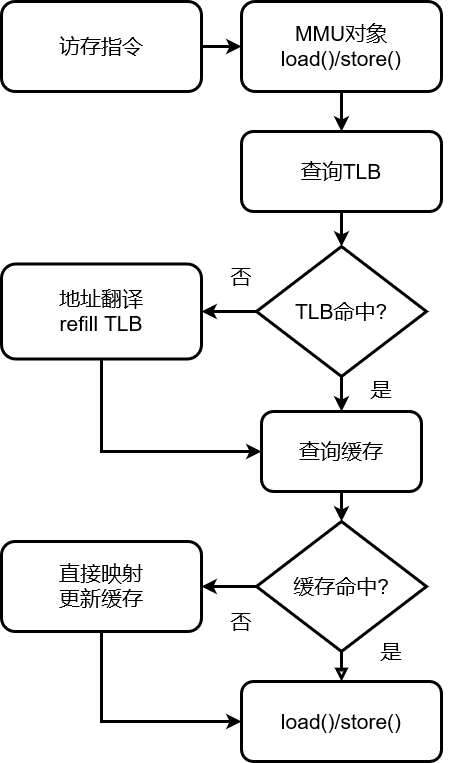
\includegraphics[width=0.45\textwidth]{mmu-cache.png}
  \caption{MMU和缓存工作流程图}
  \label{fig:mmu-process}
\end{figure}


寄存器组的模拟需要参照汇编指令具体功能进行设计。单从数据层面上讲,寄存器组只是处理器内部的一组可随机存取的数据单元,实现上使用数组就可以模拟,但是对寄存器的操作是和汇编指令功能密切相关的,RISC-V指令级架构的设计充分发挥了后发优势,将寄存器id映射到指令操作码的固定位置,从硬件设计上来讲能够极大地简化电路设计,从软件模拟的角度讲,也更加方便于接口设计,使得后续的指令集功能函数实现能够逻辑清晰,实现起来代码逻辑也更加简洁。


对于总线的模拟,可以将其抽象成统一的通信中转信箱,由全局的模拟器对象维护,可以忽略实际总线的电气特性细节,对处理器核表现为统一的外设控制器,处理包括中断控制器,RTC,BootRom固件等的以内存映射方式寻址的外部设备的通信。

\subsection{中断控制器}
上一小节介绍了CPU指令流程控制的设计,主要是取值/译码/执行的逻辑控制流程,而异常控制流,也就是中断逻辑,需要对中断控制器进行模拟,下面将介绍中断控制器模块的整体设计。本模拟器参照了SiFive公司的PLIC规范文档进行设计,通过设备树挂载PLIC设备,通过对内存映射的寄存器进行读写来配置PLIC。图~\ref{fig:plic-core}是SiFive公司给出的PLIC规范框架图。
\begin{figure}[H]
    \centering
    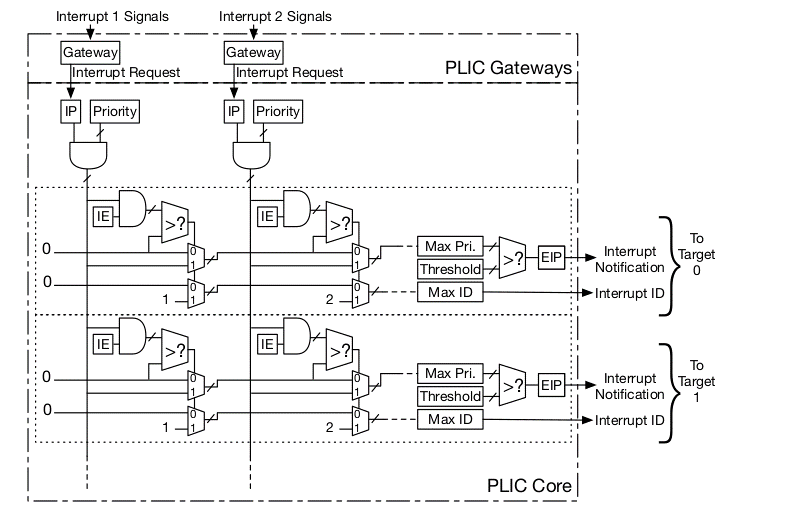
\includegraphics[width=1.0\textwidth]{plic-core.png}
    \caption{SiFive公司的PLIC框架}
    \label{fig:plic-core}
\end{figure}


中断源(interrupt sources)是挂载在PLIC上的设备的统称,一般是I/O设备。PLIC理论上支持任意多个中断源,每个中断源分配有如下的信息:


1) 闸口(Gateway)和IP(interrupt pending)。闸口控制中断源发送中断请求。IP标识当前中断源是否有请求。IP拉高时,闸口不再接受该中断源的请求。


2) 设备编号ID。PLIC为每个中断源分配的唯一编号ID。该ID也作为在多个中断源具有相同优先级时的选择条件,数值较小优先级更高。


3) 优先级(Priority)。每个中断源都有一个内存映射的Priority寄存器,表示该中断源的优先级,软件可以通过配置(设备树)将其设置成不同的优先级。优先级的数字越大,表示优先级越高。


4) 中断使能(Interrupt Enabled, IE)。每个中断源均分配了一个内存映射的中断使能寄存器,和优先级一样也可以通过设备树进行配置。IE寄存器配置为0表示该中断源被中断目标屏蔽,反之则是使能。


中断目标(interrupt targets)对应为RISC-V处理器核心的各个特权级模式。PLIC产生的外部中断请求会分别标示在处理器的mip寄存器的meip/seip位,对应于机器模式和监管模式。每个中断目标都有对应的内存映射的优先级门限(priority threshold)寄存器,只有中断源优先级高于该门限,PLIC才会将中断源ID发送给对应中断目标。


PLIC Core负责所有中断请求的仲裁和分发。图~\ref{fig:plic-process}展示了PLIC处理外部中断的流程。
\begin{figure}[h]
    \centering
    
\includegraphics[width=0.9\textwidth]{plic-process.png}
    \caption{PLIC中断处理流程}
    \label{fig:plic-process}
\end{figure}

首先,对于中断模块的被动响应方,处理器核对于中断信号的响应需要在单个指令执行周期内完成,所以模拟器在单条汇编指令的取值动作之前将对处理器核的状态寄存器进行检查,判断当前是否有待处理的中断信号,然后完成相应的硬件动作;其次,对于外部中断的主动发起方,PLIC需要进行多个外部中断源的优先级裁决,控制中断源的使能情况,并对所有处理器核的优先级门限进行筛查,对符合条件的所有中断目标发起外部中断请求。PLIC连接到模拟器的所有处理器核心,对内表现为黑盒,处理器不关心中断控制器的内部逻辑,只针对相应的外部中断信号,以及最高优先级中断源ID,进行对应的中断响应。本模拟器按照SiFive公司给出的PLIC规范文档进行设计,具体的实现将在下一章介绍。该硬件模块对处理器核表现为黑盒,只提供固定功能的接口,整体作为外部设备通过总线与处理器进行通信。

\subsection{交互调试模块}
本模拟器的主要功能就是进行目标程序的调试工作,包括Bootloader,Linux内核,驱动程序等。因此本模拟器的设计不仅需要提供丰富的调试手段,还要能够提供友好的可视化界面,方便进行目标程序调试,缩短系统软件的开发,测试,迭代周期。调试模块的功能集成在上述的处理器指令流程控制模块以及前端UI模块之中。其中,UI模块的可视化界面提供调试信息的设置,查询功能,后端模拟器指令执行流程中将对设置的调试信息进行匹配,将断点匹配结果,调试查询结果反馈到前端UI模块,与开发人员进行调试交互。该模块需要提供断点设置,单步执行,寄存器/内存查询等功能。UI显示界面主要包含了断点设置窗口,查询窗口和执行交互窗口。模拟器前后端整体的工作流程如图\ref{fig:work-frame}所示。
\begin{figure}[H]
  \centering
  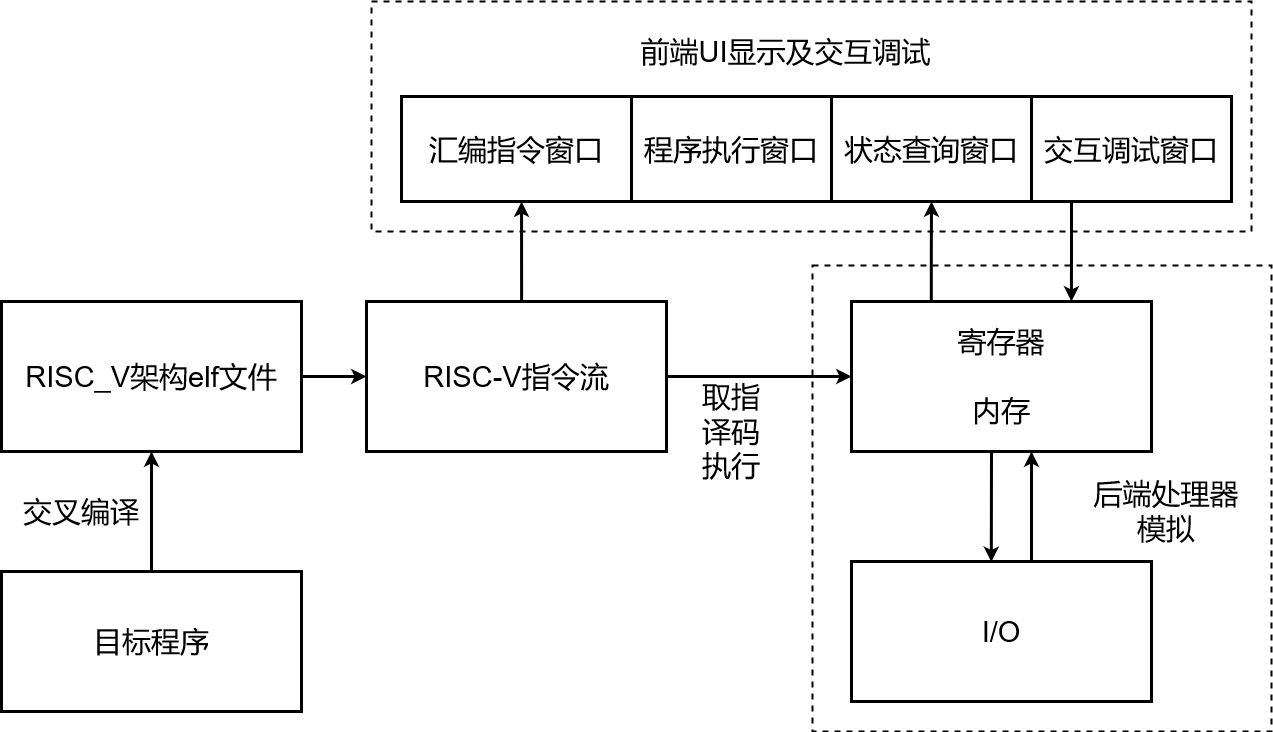
\includegraphics[width=0.8\textwidth]{sim-process.png}
  \caption{模拟器整体工作流程图}
  \label{fig:work-frame}
\end{figure}

\section{本章小结}
本章主要是根据系统的需求规格说明书,对RISC-V指令集模拟器进行概要设计,确定了本模拟器的四个主要功能模块:指令集模块,CPU和总线模块,中断模块,以及交互调试模块。描述了模拟器整体运行流程,并对各模块的功能逻辑进行设计,明确了RISC-V指令集模拟器的总体框架,动态流程以及各模块设计方案。